\documentclass[conference]{IEEEtran}
\IEEEoverridecommandlockouts
% The preceding line is only needed to identify funding in the first footnote. If that is unneeded, please comment it out.
\usepackage{cite}
\usepackage{amsmath,amssymb,amsfonts}
\usepackage{algorithmic}
\usepackage{graphicx}
\usepackage{textcomp}
\usepackage{xcolor}
\def\BibTeX{{\rm B\kern-.05em{\sc i\kern-.025em b}\kern-.08em
    T\kern-.1667em\lower.7ex\hbox{E}\kern-.125emX}}
    
    
\usepackage{ucs}
\usepackage[utf8x]{inputenc}
\usepackage[greek,english]{babel}
\newcommand{\en}{\selectlanguage{english}}
\newcommand{\gr}{\selectlanguage{greek}}    

\usepackage{wrapfig}    

\begin{document}

\title{\gr H Αλλαγή του Απορρήτου και της Διαχείρισης Δεδομένων με Επιπτώσεις στον 21\textsuperscript{o} Αιώνα\\
%{\footnotesize \textsuperscript{*}Note: Sub-titles are not captured in Xplore and
%should not be used}
%\thanks{Identify applicable funding agency here. If none, delete this.}
}

\author{\IEEEauthorblockN{ \gr ΚΙΟΥΡΤ-ΜΕΧΜΕΤΑΛΗ ΑΧΜΕΤ}
\IEEEauthorblockA{\textit{\gr Τμήμα Μηχανικών Η/Υ και Πληροφορικής} \\
\textit{\gr ΑΜ:1084672}\\
{\gr Πάτρα, Ελλάδα} \\
up1084672@upnet.gr}
\and
\IEEEauthorblockN{\gr ΣΤΑΜΑΤΟΠΟΥΛΟΣ ΘΕΜΙΣΤΟΚΛΗΣ}
\IEEEauthorblockA{\textit{\gr Τμήμα Μηχανικών Η/Υ και Πληροφορικής} \\
\textit{\gr ΑΜ:1070735}\\
{\gr Πάτρα, Ελλάδα} \\
up1070735@upnet.gr}
}

\maketitle



\gr \section*{\fontsize{17}{20}\selectfont Υπόμνημα (228)}
\gr \subsection*{\fontsize{13}{15}\selectfont Eπιλογή Άρθρων}
% \gr  \huge \textbf{Επιλογή Άρθρων}
%\end{center}

\small

\smallskip 

\gr

ΟΝΟΜΑΤΕΠΩΝΥΜΟ:ΚΙΟΥΡΤ-ΜΕΧΜΕΤΑΛΗ ΣΤΑΜΑΤΟΠΟΥΛΟΣ 
\smallskip \\
\en 

SHA-1:493c775805710e494256724bdb490ed14e0933f1
\smallskip \\
\gr

Διακριτά ψηφία: 4,9,3,7,5,8 (δεδομένου ότι η συλλογή δεν είχε άρθρο \en c)

\setlength{\arrayrulewidth}{0.5mm}
\setlength{\tabcolsep}{18pt}
\renewcommand{\arraystretch}{1.5}
\bigskip



\begin{tabular}{ |p{0.5cm}|p{4.6cm}| }


\hline
4& What is Überveillance? (And What Should Be Done  About It?) \\
\hline
9& Big Data ethics \\
\hline
3& Mimetic Models: Ethical Implications of AI that Acts Like You \\
\hline
7& Social ethics in Internet of Things:An outline and review \\
\hline
5& Ethics for Big Data and Analytics \\
\hline
8& Algorithmic amplification of politics on Twitter  \\
\hline
\end{tabular}

 \bigskip
\bigskip



\huge
\gr \subsection*{\fontsize{13}{15}\selectfont Ομάδα}

\normalsize
\begin{flushleft}
\gr Για βιβλιογραφική παρουσίαση έχουμε διαλέξει τα εξής άρθρα:\\ \en
1. What is Überveillance? (And What Should Be Done  About It? \\
2. Algorithmic amplification of politics on Twitter \\
3. Big Data ethics \\
4. Ethics for Big Data and Analytics \\

\bigskip

\gr Για Παρουσίαση \en Powerpoint \gr και για Συζήτηση με το \en ChatGPT \gr διαλέξαμε το άρθρο \en Big Data ethics \gr που είναι το 2ο άρθρο του αλγόριθμου.

\bigskip


Ως ομάδα αρχικά προσπαθήσαμε να καταλάβουμε τα άρθρα και να επιλέξουμε τα καλύτερα που θα έχει το αποτέλεσμα της καλύτερης συνεννόησης μεταξύ των μελών. Στην συνέχεια δεν επιλέξαμε το 2ο ή το 3ο άρθρο από το \en SHA-1 \gr για να μην υπάρχει ομοιότητα στις αναφορές που θα παρουσιάσουμε. Υπήρξαν περιπτώσεις που δεν είχαμε καταλάβει καλά την έννοια του κειμένου που ρωτάγαμε ο ένας τον άλλων. 
Για την παρουσίαση του άρθρου, διαβάσαμε ξεχωριστά το άρθρο έτσι ώστε να έχουμε και διαφορετικές απόψεις που αυτή η λεπτομέρεια μας βοήθησε σε δημιουργία των διαφάνειων.   
\end{flushleft}




\en
\begin{abstract}
\gr \section*{\fontsize{17}{20}\selectfont Περίληψη (190)}
\gr
Από της αρχές του 21ο αιώνα και της ανάπτυξης της τεχνολογίας δυστυχώς το απόρρητο έχει σχεδόν εξαφανιστεί. Με τις έννοιες ότι η μυστικότητα και η προσωπική ζωή της κοινωνίας να είναι σε κίνδυνο. Η ελευθερία και η σκέψη εξαρτάται από τους αλγόριθμους που καθοδηγεί τον καθέναν μας σε μία σκέψη ανάλογα με τα «κλικ» του παρελθόν. Η επιτήρηση δεν γίνεται μόνο με τρόπους του 20ου αιώνα αλλά και με ένα ποιο σύγχρονο τρόπο με δεδομένα. Με πολλές ενέργειες που δεν διατηρεί την ηθικότητα που θα χρειαζόταν. Βέβαια, υπάρχουν και περιπτώσεις που τα δεδομένα ακόμα και σώζουν ζωές αλλά και βοηθούν σε ανάπτυξη της επιστήμης. Αν και δεν υπάρχει μία καθαριότητα σχετικά με τους αλγόριθμους που χρησιμοποιούνται στα κοινά δίκτυα, το δημόσιο έχει μία καλύτερη επεξήγηση στο απόρρητο. Για αυτό και μόνον λόγο πρέπει να υπάρξουν νέους οργανισμούς στο μέλλον μόνο και μόνο να διαπιστώνουνε με ένα ορθό τρόπο όλες τις διαδικασίες για να ξεφύγουμε αυτό το τεράστιο ερωτηματολόγιο. Τέλος, τα δεδομένα που χρησιμοποιούνται  για πάρα πολλούς διαφορετικούς λόγους είναι φανερό ότι θα δημιουργήσουν μία νέα επανάσταση στο κοντινό μέλλον με της ανάπτυξης της τεχνητής νοημοσύνης καθημερινά.
\end{abstract}

\begin{IEEEkeywords}
\gr δεδομένα, μέλλον, απόρρητο, ηθικότητα
\end{IEEEkeywords}



\newpage

\gr \section*{\fontsize{17}{20}\selectfont Βιβλιογραφική Παρουσίαση (1284)}


\small
\en \subsection*{\fontsize{13}{15}\selectfont \en What is Überveillance?(And What Should Be Done About It?)}
\normalsize
\gr

Η εξελισσόμενη επιτήρηση των ατόμων αποτελεί κεντρικό κίνδυνο, η μετάβαση από τις φυσικές σε αυτοματοποιημένες μεθόδους που παραβιάζουν την ιδιωτική ζωή. Με τις τηλεπικοινωνιακές εξελίξεις, η επιτήρηση δεδομένων έχει αναδειχθεί ως ένα ευρέως διαδεδομένο και οικονομικά αποδοτικό εργαλείο, που περιλαμβάνει την παρακολούθηση των σκέψεων και την επικοινωνία, εγείροντας ανησυχίες στο κοινό.

Η εμφάνιση του \en “Uberveillance” \gr και του \en “Omni-Surveillance”, \gr τα οποία έχουν μειώσει σημαντικά το απόρρητο παρακολουθώντας συνεχώς τα άτομα μέσω τεχνολογιών όπως τα \en chip \gr και τα καλώδια. Εν τω μεταξύ, η \en "Sureveillance" \gr έχει εξελιχθεί σε ένα ισχυρό εργαλείο για την ανίχνευση εγκλημάτων, αλλά η διαχείριση του τεράστιου όγκου δεδομένων που δημιουργείται παρουσιάζει προκλήσεις.

Για να αντιμετωπίσουμε αυτά τα ζητήματα, χρειαζόμαστε ανεξάρτητη επιστημονική έρευνα και πειράματα σε αυτήν την τεχνολογία, απαλλαγμένα από την επιρροή χωρών όπως οι ΗΠΑ και η Αυστραλία. Αυτό θα διασφαλίσει ότι το κοινό ενημερώνεται για τον σχεδιασμό και τις ιδιότητες του συστήματος, παρέχοντάς του τόσο την ελευθερία όσο και τη δυνατότητα να διαμορφώνουν τις δικές τους σκέψεις.

Συμπερασματικά, η ισορροπία στην επιτήρηση και ασφάλεια είναι ένα φανερό συμπέρασμα για μία κατάλληλη ζωή. Είναι φανερές ότι πρέπει να γίνει μία νέα οργάνωση στην νομοθεσία λόγο τις απώλειες λόγο του αιώνα που ζούμε για μία κατάλληλη ζωή που η μυστικότητα σχεδόν δεν υπάρχει.


\en  \subsection*{\fontsize{12}{15}\selectfont Algorithmic amplification of politics on Twitter}
\normalsize


\gr Το \en Twitter \gr είναι ένα ισχυρό εργαλείο πολιτικής προπαγάνδας. Δύο πειράματα αποκαλύπτουν ότι τα κυβερνώντα κόμματα λαμβάνουν ισχυρότερη ενίσχυση, συχνά ευνοώντας δεξιές πηγές. Ο στόχος είναι να κατανοήσουμε ποιες έννοιες λαμβάνουν υποστήριξη για πολιτικές ιδεολογίες.

To \en Control Group \gr θα είναι η ομάδα που θα διοργανώνει το πείραμα με τα δεδομένα που θα χρησιμοποιηθεί αλλά το \en Treatment Group \gr είναι η ομάδα που θα «θεραπέψει» το αλγόριθμο για να έχουμε ένα καθαρό αποτέλεσμα. Έχουμε μία μονάδα T και ένα σύνολο \en U\gr. Που θα εκτελείται ο αλγόριθμος ώστε να απαντά σε ίση αναλογική εμβέλεια και στα δύο \en groups.\gr Ώστε να δουλεύουν εναλλακτικά.

Στις περισσότερες χώρες, εκτός από τη Γερμανία, η πολιτική ικανότητα ευνοείται έναντι των κομματικών δεσμών. Σε ατομικό επίπεδο, ορισμένοι πολιτικοί βιώνουν 400\% αύξηση στην ενίσχυση μέσω \en tweets \gr, ενώ άλλοι επωφελούνται από μια χρονολογική κατάταξη. Αυτή η ατομική ενίσχυση οδηγεί σε έλλειψη μεσαίου δρόμου μεταξύ του κυβερνητικού συνασπισμού και της αντιπολίτευσης, με οριακή αύξηση της δεξιάς σκέψης. Τα μέσα ενημέρωσης μπορούν επίσης να επηρεάσουν αυτές τις δυναμικές.

Ο αλγόριθμος βασίζεται περισσότερο στα μέσα παρά στις ιδεολογίες. Η έρευνα ανέλυσε 58 εκατομμύρια χρήστες, ενώ η ομάδα θεραπείας είχε περισσότερους. Οι αξιόπιστες χώρες εντοπίστηκαν χρησιμοποιώντας το \en Google \gr και το \en Yahoo. \gr Η εξίσωση προσαρμόστηκε με βάση τη χώρα.



\en \subsection*{\fontsize{13}{15}\selectfont Big Data ethics}
\normalsize
\gr
Σύμφωνα με αυτό το άρθρο, ο αρθρογράφος περιγράφει τις παραδοσιακές ηθικές αρχές όσον αφορά την ηθική ευθύνη, έπειτα συνεχίζει με τις τέσσερις ιδιότητες των Μεγάλων Δεδομένων με ηθική συνάφεια. 

Εμβαθύνει στην ιδέα της μεταβαλλόμενης φύσης της εξουσίας και της εμφάνισης της υπερδικτυωμένης ηθικής, και επεξηγεί ποια ηθικά προβλήματα ενδέχεται να προκύψουν στην κοινωνία, την πολιτική και την έρευνα λόγω αυτών των αλλαγών. Εξηγεί, ότι η ηθική των Μεγάλων Δεδομένων απομακρύνεται από έναν προσωπικό ηθικό παράγοντα σε ορισμένες περιπτώσεις. Σε άλλες περιπτώσεις, αυξάνει την ηθική ευθύνη όσων έχουν τον έλεγχο των Μεγάλων Δεδομένων. Γενικά, η τάση είναι προς μια απρόσωπη ηθική που βασίζεται σε συνέπειες για τους άλλους. Ωστόσο, παρατηρεί ότι υπάρχουν μερικές ηθικές προκλήσεις με τα Μεγάλα Δεδομένα, όπως την παραβίαση της ιδιωτικότητας των ατομικών ή ομαδικών προσωπικών στοιχείων στο διαδίκτυο και την αδυναμία της αποτροπής σοβαρών εγκλημάτων στην κοινωνία.

Τέλος, αναφέρει την ηθική των Μεγάλων Δεδομένων, δεν φαίνεται να είναι υπερεκτίμηση να πούμε ότι τα Μεγάλα Δεδομένα έχουν όντως ισχυρές επιπτώσεις στις υποθέσεις σχετικά με την ατομική ευθύνη και την κατανομή ισχύος. Συμπερασματικά, για να λυθούν τα προβλήματα αυτά, πρέπει να συνεχίσουμε να συζητούμε πώς μπορούμε και πώς θέλουμε να ζούμε σε έναν κόσμο με δεδομένα και πώς μπορούμε να αποτρέψουμε την κατάχρηση των Μεγάλων Δεδομένων ως νέας πηγής πληροφοριών και δύναμης.


\en \subsection*{\fontsize{13}{15}\selectfont Ethics for Big Data and Analytics}
\normalsize
\gr
 Σ' αυτό το άρθρο, εξηγείται ότι η ηθική των υπολογιστών έχει μια κληρονομιά κτίζοντας σε αυτό το υπόστρωμα, με σημαντική που εξετάζει βασικά σχετικά ζητήματα. Σαν αποτέλεσμα, μάλλον δεν αποτελεί έκπληξη το γεγονός ότι υπάρχουν πολλά ορισμοί, και κάποια διαμάχη, ως προς το ποια διαφωνία θεσπίζει την ηθική των υπολογιστών.
 
 Συγκεκριμένα, η ηθική και η ηθική των υπολογιστών εκδηλώνονται σε ο κόσμος ως «κώδικες ηθικής» και «κώδικες συνθηκών αγωγός» που αναπτύχθηκε από διαφορετικούς οργανισμούς. Η ύπαρξη ενός κώδικας δεοντολογίας ή συμπεριφοράς παρέχει ένα μήνυμα ως όπου μια τεχνολογία βρίσκεται στον κύκλο ζωής της. Έτσι, η ανάπτυξη κωδίκων δεοντολογίας υποδηλώνει χρήση μιας τεχνολογίας και ανάπτυξη ενός συνόλου κανόνων προς έλεγχο αυτή η συμπεριφορά χρήσης. Επειδή υπάρχει διαμάχη με την ηθική σε σύγκριση με τη γενική ηθική πλαίσια , μπορεί να υπάρξει μια αντιπαράθεση για τα ζητήματα όπως αν τα δεδομένα και τα αναλυτικά στοιχεία ανήκουν στον υπολογιστή ηθική ή εάν πρέπει να αντιμετωπίζονται τα δικά τους. H ηθική των δεδομένων διαφέρει από την ηθική των υπολογιστών, όπως φαίνεται από τις διαφορές ανάμεσα στα τεχνουργήματα, το διαφορετικό αναδυόμενοι κώδικες ηθικής, και η έλλειψη ιδιαιτερότητας σε υπολογιστές ή γενικά ηθικά πλαίσια.
 
 Όμως, τέτοια όρια μπορούν σπάνια να προβλέπουν πλήρως αυτό που οι άνθρωποι μπορεί να δημιουργήσουν ή πώς μπορεί να είναι πρέπει μέχρι μια δεδομένη τεχνολογία να έρχεται πιο πλήρως ανεπτυγμένη. Επιπλέον, τέτοια οριοθέτηση σε μεγάλο βαθμό αγνοεί πιθανές θετικές κατευθυντήριες γραμμές ή προτάσεις.


\en \subsection*{\fontsize{13}{15}\selectfont \gr Κριτική Συζήτηση με το \en ChatGPT}
\gr \underline{Ερώτηση:} Δώστε μία περίληψη του άρθρου \en Big Data Ethics \gr του συγγραφέα \en Andrej Zwitter
\bigskip \\
\gr \underline{Απάντηση:} Το άρθρο \en "Big Data Ethics" \gr του συγγραφέα \en Andrej Zwitter \gr αναφέρεται στην ηθική διάσταση της ανάπτυξης και χρήσης των μεγάλων δεδομένων. Ο συγγραφέας εξετάζει τις ηθικές προκλήσεις που προκύπτουν από τη συλλογή, αποθήκευση, επεξεργασία και ανάλυση τεράστιων ποσοτήτων δεδομένων.

Αρχικά, αναλύει την έννοια των μεγάλων δεδομένων και τη σημασία τους για την τεχνολογία, την κοινωνία και την οικονομία. Εξετάζει τα πλεονεκτήματα που προκύπτουν από την αξιοποίηση των μεγάλων δεδομένων, όπως η πρόοδος στην επιστήμη, η καινοτομία και η βελτίωση των υπηρεσιών.

Ωστόσο, ο \en Zwitter \gr επισημαίνει ότι η ανάπτυξη των μεγάλων δεδομένων συνεπάγεται και ηθικά ζητήματα που πρέπει να αντιμετωπιστούν. Αναφέρει πρώτον το ζήτημα της ιδιωτικότητας και της προστασίας των προσωπικών δεδομένων, καθώς η συλλογή και ανάλυση τεράστιων ποσοτήτων δεδομένων μπορεί να παραβιάσει την ιδιωτική ζωή των ανθρώπων.
\bigskip \\

\gr \underline{Ερώτηση:} Τι λέει το άρθρο για το κομμάτι \en New Power Distributions \gr του άρθρου \en Big Data Ethics \gr του συγγραφέα \en Andrej Zwitter;
\bigskip \\
\gr \underline{Απάντηση:}Λυπάμαι για την παρεξήγηση, αλλά δεν έχω πρόσβαση σε συγκεκριμένο άρθρο του \en Andrej Zwitter \gr με τον τίτλο \en "Big Data Ethics".\gr Ως γλωσσικό μοντέλο AI, δεν έχω τη δυνατότητα να αναζητήσω πληροφορίες σε πραγματικό χρόνο ή να παράσχω απευθείας περιεχόμενο από το συγκεκριμένο άρθρο.


\en \subsection*{\fontsize{13}{15}\selectfont \gr Εντυπώσης των απαντήσεων του \en ChatGPT}
\gr Παρατηρούμε ότι στην πρώτη ερώτηση μας απαντάει χωρίς να έχει αναλύσει το συγκεκριμένο άρθρο και απαντάει ότι το άρθρο αναφέρεται για οικονομία που είναι λάθος. 

Στην δεύτερη ερώτηση που έχουμε κάνει είναι προφανές ότι η απάντηση που μας δίνει λάθος με το γεγονός να μην μπορεί να απαντήσει ακόμα και με ένα άσχετο τρόπο.
\bigskip \\
\gr Τέλος, μπορούν να μελετηθούν και άλλες ενδιαφέρουσες πηγές για το θέμα όπως:\\
\en 1. A research note on ethics in the emerging age of Überveillance\\
2.Critiquing Big Data: Politics, Ethics, Epistemology\\
3.What is Überveillance? (And What Should Be Done About It?)\\
4.Ethics for Big Data and Analytics\\
5.AI Rewrites Coding\\
6.Social ethics in Internet of Things:An outline and review\\
7.Algorithmic amplification of politics on Twitter\\
8.Freedom and privacy in Ambient Intelligence\\
9.The ethics of algorithms: key problems and solutions\\

\en \subsection*{\fontsize{13}{15}\selectfont \gr Συζήτηση}

\gr 
Το απόρρητο, η ηθικότητα και τα δεδομένα είναι οι τρεις λέξεις που θα διαμορφώσουν το μέλλον μας. Κατά την γνώμη μας τα άρθρα είναι μία καθοδήγηση και προετοιμασία για τα γεγονότα που θα ζήσουμε. Ως κοινό πρέπει να ξέρουμε και να είμαστε σε επιφύλαξη με τις νέες περιπτώσεις που θα προκύψουν στη ζωή μας θετικά αλλά και αρνητικά.







\gr \section*{\fontsize{17}{20}\selectfont Βιβλιογραφία}

\en 1. Michael M. G., Fusco Sarah Jean and Michael Katina (2008): A research note on ethics in the emerging age of Überveillance.School of Information Systems and Technology, Faculty of Informatics, University of Wollongong, P.O. Box U184, Wollongong, NSW 2522, Australia
\textcolor{blue}{https://ro.uow.edu.au/infopapers/583} \\ 

2. Kate Crawford, Kate Miltner and Mary L. Gray (2004): Critiquing Big Data: Politics, Ethics, Epistemology. International Journal of Communication 8 (2014), 1663–1672. ISSN:1932–8036/20140005 \\

3. Reid McIlroy-Young, Jon Kleinberg, Siddhartha Sen, Solon Barocas and Ashton Anderson (2022): Mimetic Models: Ethical Implications of AI that Acts Like You. AIES ’22, August 1–3, 2022, Oxford, United Kingdom \\

4. Roger Clarke (2010):What is Überveillance? (And What Should Be Done About It?). IEEE Technology and Society Magazine 29(2):17 - 25 DOI:10.1109/MTS.2010.937030.Source:IEEE Xplore \\

5. Daniel E. O’Leary (2016): Ethics for Big Data and Analytics.IEEE Intelligent Systems ( Volume: 31, Issue: 4, July-Aug. 2016) DOI:10.1109/MIS.2016.70 \\

6. Samuel Greengard (2023): AI Rewrites Coding. Communications of the ACM, April 2023, Vol. 66 No. 4, Pages 12-14 DOI:10.1145/3583083 \\

7. Amin Shahraki and Øystein Haugen (2018): Social ethics in Internet of Things:An outline and review. 2018 IEEE Industrial Cyber-Physical Systems (ICPS) DOI: 10.1109 ICPHYS.2018.8390757 \\

8. Ferenc Huszár, Sofia Ira Ktena, Conor O’Brien, Luca Belli, Andrew Schlaikjer and Moritz Hardt (2021): Algorithmic amplification of politics on Twitter. PNAS(Proceedings of the National Academy of Sciences of the United States of America) DOI: 10.1073/pnas.2025334119 \\ 
9. Andrej Zwitter (2014): Big Data Ethics. Big Data \& Society July–December 2014: 1–6 DOI:10.1177/2053951714559253 \\

10. Philip Brey (2006): Freedom and privacy in Ambient Intelligence. Ethics and Information Technology (2005) 7:157–166 DOI:10.1007/s10676-006-0005-3 \\

11. Andreas Tsamados, Nikita Aggarwal, Josh Cowls, Jessica Morley, Huw Roberts, Mariarosaria Taddeo and Luciano Floridi (2021):The ethics of algorithms: key problems and solutions. AI \& SOCIETY (2022) 37:215–230 \textcolor{blue}{https://doi.org/10.1007/s00146-021-01154-8}




\gr \section*{\fontsize{17}{20}\selectfont Βιογραφικά (184)}



\begin{wrapfigure}{l}{0.18\textwidth}
  \centering
  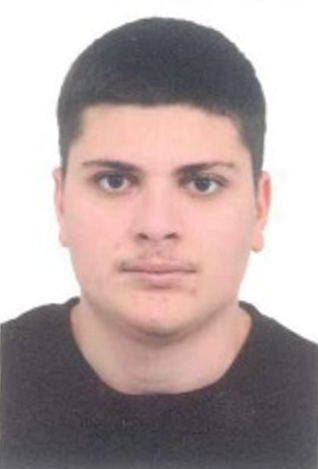
\includegraphics[width=0.980\linewidth]{photo.png}
\end{wrapfigure}

\normalsize

\gr Ο Κιουρτ-Μεχμεταλή Αχμέτ είναι προπτυχιακός φοιτητής (έτος εισαγωγής: 2020) του τμήματος Μηχανικών Ηλεκτρονικών Υπολογιστών και Πληροφορικής του Πανεπιστημίου Πατρών. Εθελοντής σε πολλές εργασίες όπως με τίτλο «Εξέλιξη Πολιτισμού» στη δευτεροβάθμια εκπαίδευση για να αποκτήσει δεξιότητες επικοινωνίας. Γνωρίζει σε πολύ καλό επίπεδο Αγγλικά και Τουρκικά (με πτυχία). Με υψηλά κίνητρα ενδιαφέρεται για την εξέλιξη της τεχνολογίας ιδιαίτερα με το υλικό \en(hardware), \gr αλλά και με  \en database systems. \gr Έχει εμπειρία με εργασίες προγραμματισμού σε επίπεδο λογισμικού όπως σε γλώσσες \en C,C++,SQL,Java.\gr  Στο υλικό συγκεκιρμένα απασχολείτε με \en IC (Integrated Circuit), Verilog \gr και \en System Verilog.

\newpage
 \bigskip
 

\begin{wrapfigure}{l}{0.18\textwidth}
  \centering
  
\includegraphics[width=0.980\linewidth]{image2.png}
\end{wrapfigure}

\gr Ο Θεμιστοκλής Σταμαπόπουλος είναι προπτυχιακός φοιτητής του τμήματος Μηχανικών Ηλεκτρονικών Υπολογιστών και Πληροφορικής του Πανεπιστημίου Πατρών. Έχει δεξιότητες στο προγραμματισμό όπως σε \en C/C++, Java, x86 Assembly, JavaScript, HTML \gr και \en CSS. \gr Γνωρίζει την χρήση των λειτουργικών συστημάτων όπως \en Windows, Linux \gr και \en Ubuntu. \gr Έχει εργασιακή  εμπειρία ως \en Ligua Expert \gr στο τμήμα εκμάθησης Αγγλικών και Πληροφορικής για θέμα διδακτική πείρα στα μαθήματα Αγγλικών και Πληροφορικής σε μαθητές δημοτικού, γυμνάσιου και λυκείου όπως και για το θέμα ανάπτυξη εφαρμογών σε διάφορα περιβάλλοντα και λειτουργικά συστήματα \en(Windows, Ubuntu)




\end{document}
